\appendix
%\renewcommand{\appendixname}{Appendix~\Alph{chapter}}
\chapter{Accelerator Models}
Hardware resource on FPGA mainly includes DSP, LUT, FF and BRAM (block RAM). LUT, FF and DSP consumption can be roughly estimated with a linear function of SCGRA size and can be calculated using \eqnref{eq:dsplutff}. BRAM consumption $ResConsumption(\bm{C}, 1)$ which is slightly different from LUT, FF and DSP consumption can be calculated precisely based on the memory block configurations. 
\begin{equation} \label{eq:dsplutff}
    ResConsumption(\bm{C}, i)=\alpha_i \times r \times c + \beta_i, (i=2,3,4)
\end{equation}

Power consumption is consisted of block RAM power, clock power, signal power, DSP power and so on according to the XPower report. The block BRAM power consumption shows very good linearity with the amount of block RAM consumption while the rest part of the power is linear to the SCGRA size. Thus the power consumption can be calculated by \eqref{eq:power}. 

\begin{equation}\label{eq:power}
Power(\bm{C}) = ResConsumption(\bm{C}, 1) \times \alpha_5 + \alpha_6 \times r \times c + \beta_5
\end{equation}

With the performance and power models, the energy consumption which is the production of power and loop execution time can be obtained using \eqnref{eq:energy}. Finally, energy efficiency represented by energy delay product which is the production of energy consumption and loop execution time can be calculated using \eqnref{eq:edp}.

\begin{equation} \label{eq:energy}
Energy(\bm{C}) = Power(\bm{C}) \times RunTime(\bm{C}) / f
\end{equation}

\begin{equation} \label{eq:edp}
EDP(\bm{C}) = Energy(\bm{C}) \times RunTime(\bm{C}) / f
\end{equation}

\chapter{Accelerator Implementation Analysis}
In order to analyze the FPGA resource consumption and power consumption of the SCGRA overlay based FPGA accelerators, three groups of accelerators including SCGRA1, SCGRA2 and SCGRA3 with various configurations as detailed in \tabref{tab:config} are implemented on Zedboard. Based on the implementation results, the FPGA resource consumption and power consumption are analyzed respectively in the section.

\begin{table}[htb]
    \footnotesize
    \centering
    \caption{SCGRA Based FPGA Accelerator Configuration \label{tab:config}}{
        \begin{tabular}{c|c|c|c|c|c}
            \hline
            Group & Size & \tabincell{c}{Inst. \\ Rom} & 
            \tabincell{c}{Data \\ Mem} & \tabincell{c}{IBuf \\ /OBuf} & 
            \tabincell{c}{Addr \\Buf} \\ \hline

            SCGRA1 & \tabincell{l}{2x2, 3x2, \\ 3x3, 4x3, \\ 4x4, 5x4} & 
            1kx72 & 256x32 & 2kx32 & 4kx16\\ \hline

            SCGRA2 & \tabincell{l}{2x2, 3x2, \\ 3x3, 4x3, \\4x4} & 
            2kx72 & 256x32 & 2kx32 & 4kx16\\ \hline

            SCGRA3 & \tabincell{l}{2x2, \\ 3x2, \\ 3x3 } &  
            4kx72 & 256x32 & 2kx32 & 4kx16\\ \hline
        \end{tabular}
    }
\end{table}

\figref{fig:SCGRA-Overhead} shows the relation between the four types of FPGA resource consumption and SCGRA overlay size. It can be found that the consumption of FF, LUT and DSP does not change much with the memory configurations and they present very good linearity to the SCGRA overlay size. Therefore, they can be estimated with linear models. Block RAM consumption depends on both the overlay size and the memory configurations, and single variable linear model will not work for the estimation. Fortunately, all the memory components in the SCGRA overlay are implemented using primitive block RAMs and they can be calculated precisely with the memory configurations. 

\begin{figure}[tb]
\centering
    \subfigure[\label{fig:FF-Overhead}]{%
      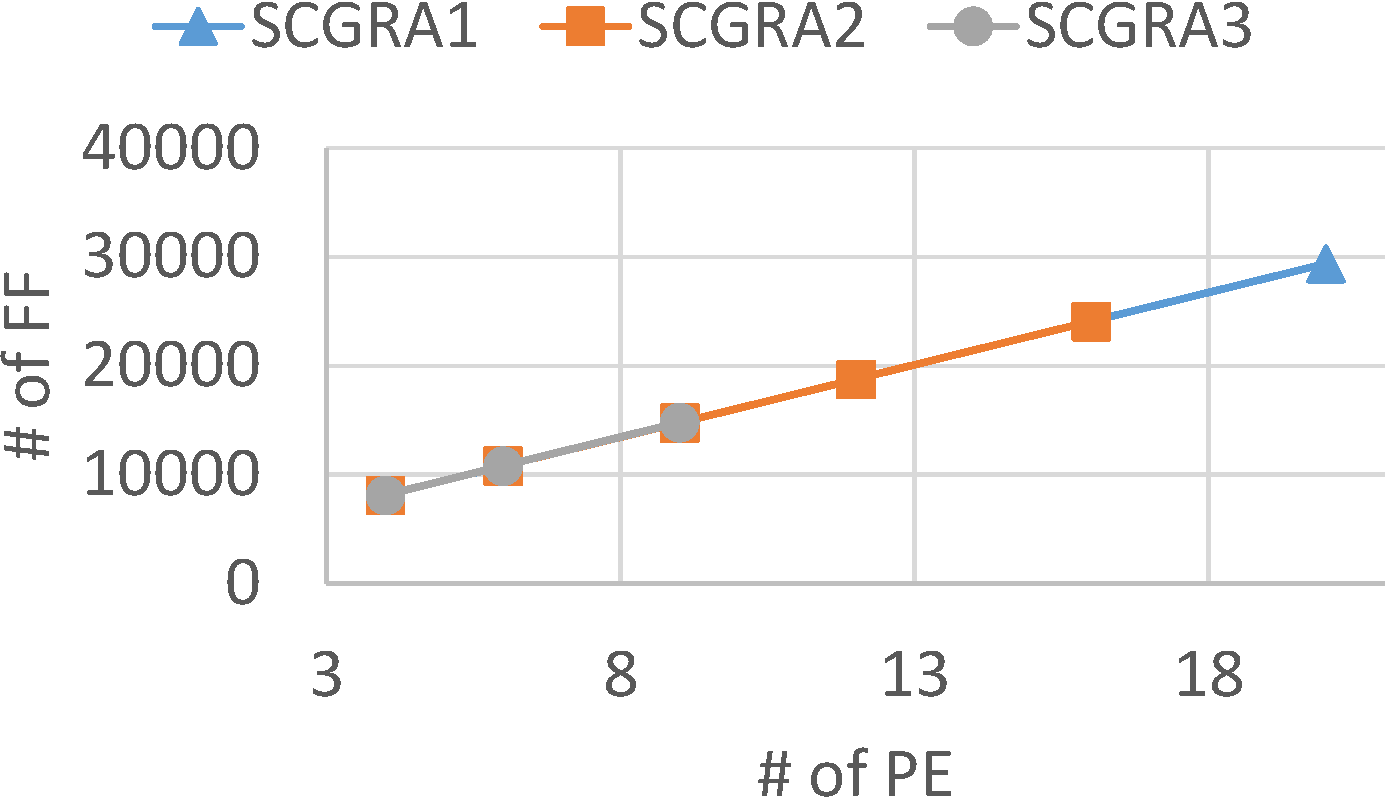
\includegraphics[width=0.45\textwidth]{FF-Overhead}
    }
    \subfigure[\label{fig:LUT-Overhead}]{%
      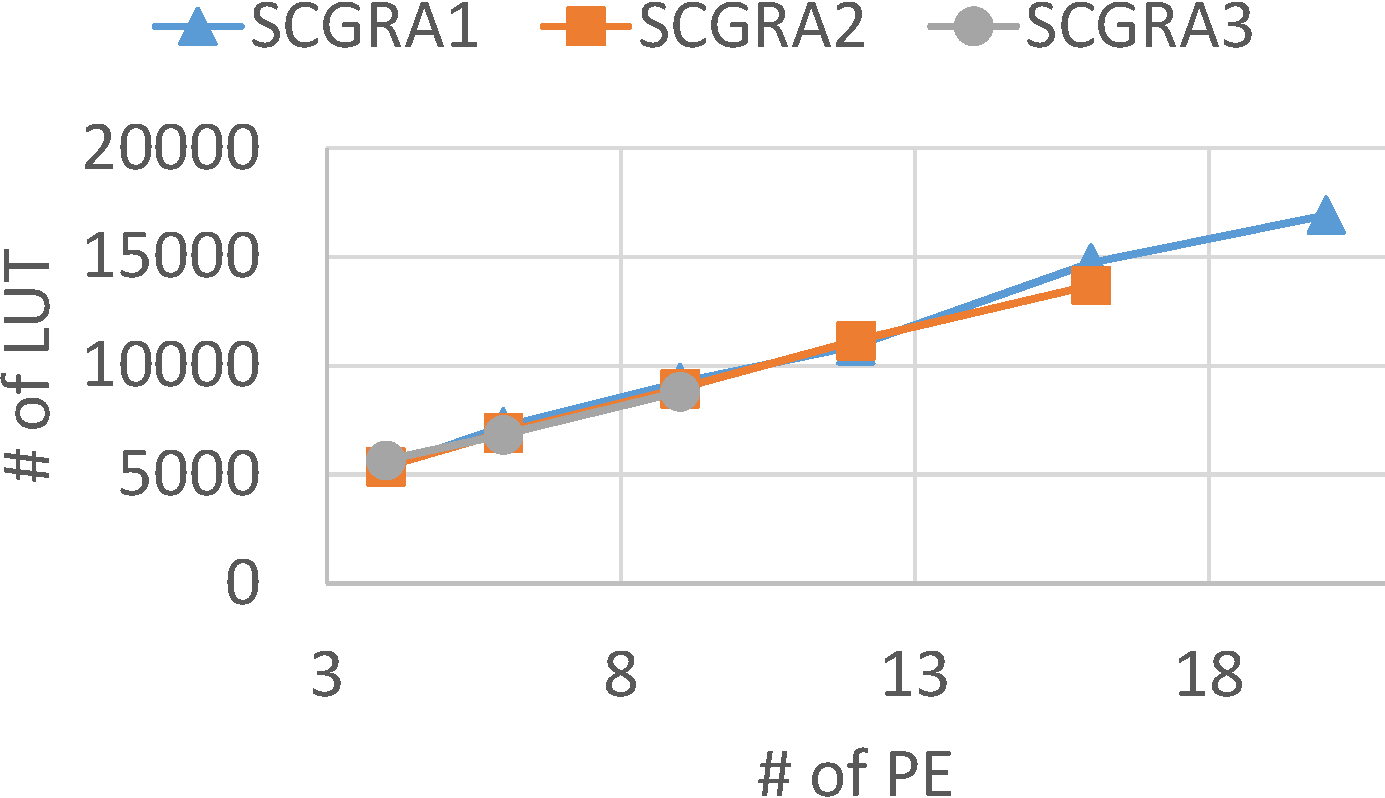
\includegraphics[width=0.45\textwidth]{LUT-Overhead}
    }
    \hfill
    \subfigure[\label{fig:DSP-Overhead}]{%
      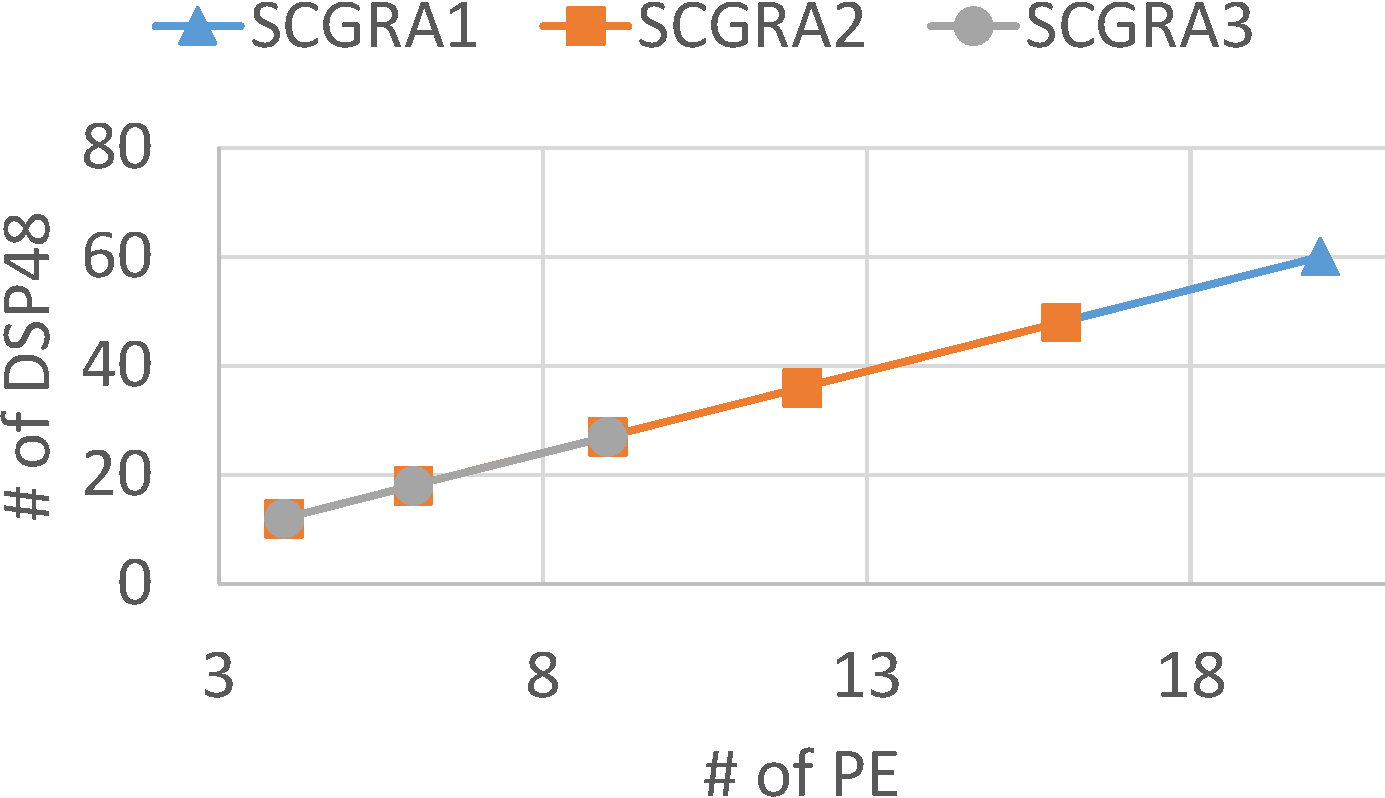
\includegraphics[width=0.45\textwidth]{DSP-Overhead}
    }
    \subfigure[\label{fig:BRAM-Overhead}]{%
      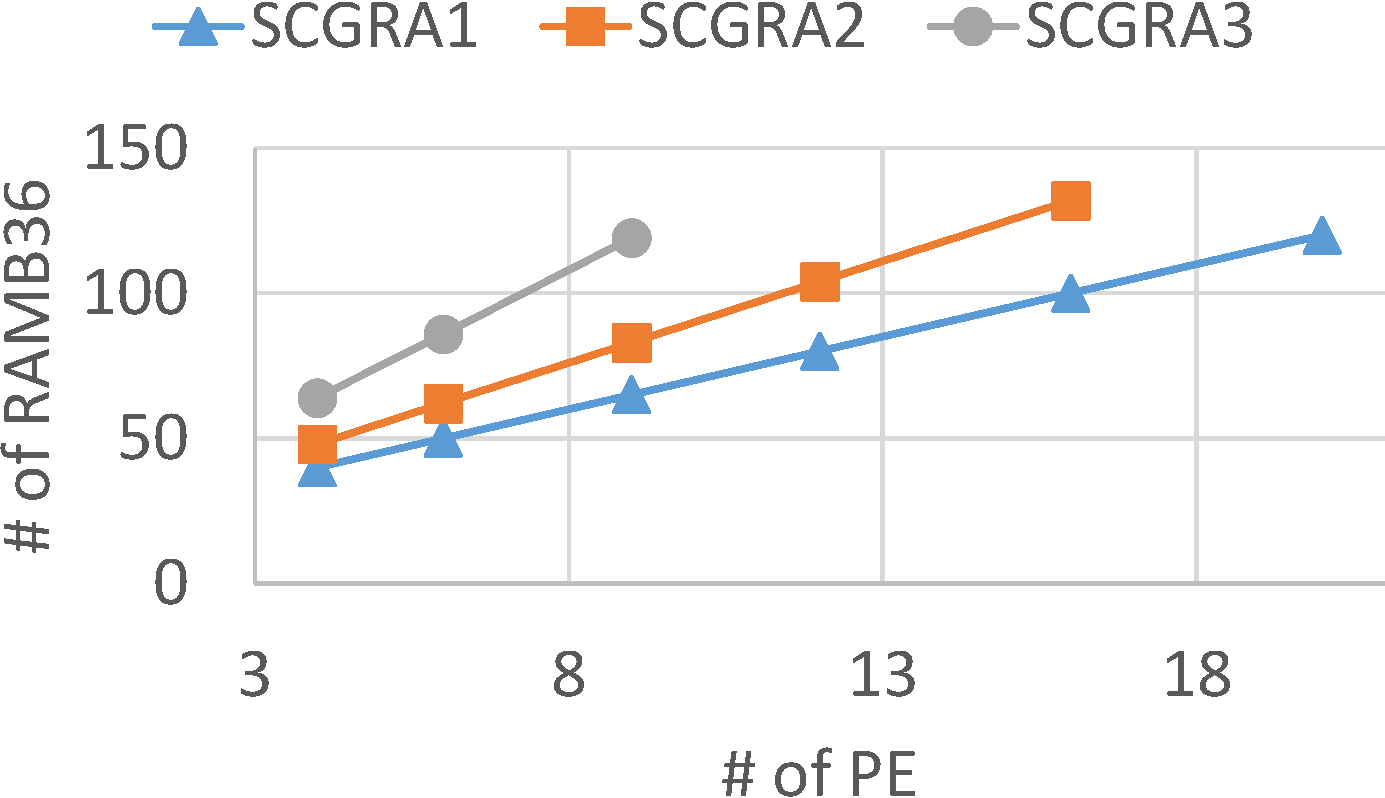
\includegraphics[width=0.45\textwidth]{BRAM-Overhead}
    }
    \caption{Relation between The Accelerators' FPGA Resource Consumption and The SCGRA Overlay Size, 
    (a) FF Consumption, (b) LUT Consumption, (c)DSP Consumption, (d)BRAM Consumption}
    \label{fig:SCGRA-Overhead}
\end{figure}

According to the power decomposition in Xpower, the power consumption of an FPGA design includes signal power, clock power, BRAM power and so on. To simplify the power model of the SCGRA overlay based FPGA accelerator, the power consumption is divided into BRAM power and base system power which essentially includes the power consumption of the rest part of the system. As shown in \figref{fig:SCGRA-Power}, the base system power exhibits good linearity over the SCGRA overlay size while the BRAM power is near linear to the BRAM consumption. As mentioned in previous paragraph, the BRAM consumption can be immediately calculated given the SCGRA overlay configuration. Therefore, both of the two parts of the power consumption can be estimated. 

\begin{figure}[htb]
\centering
    \subfigure[\label{fig:Base-Power}]{%
      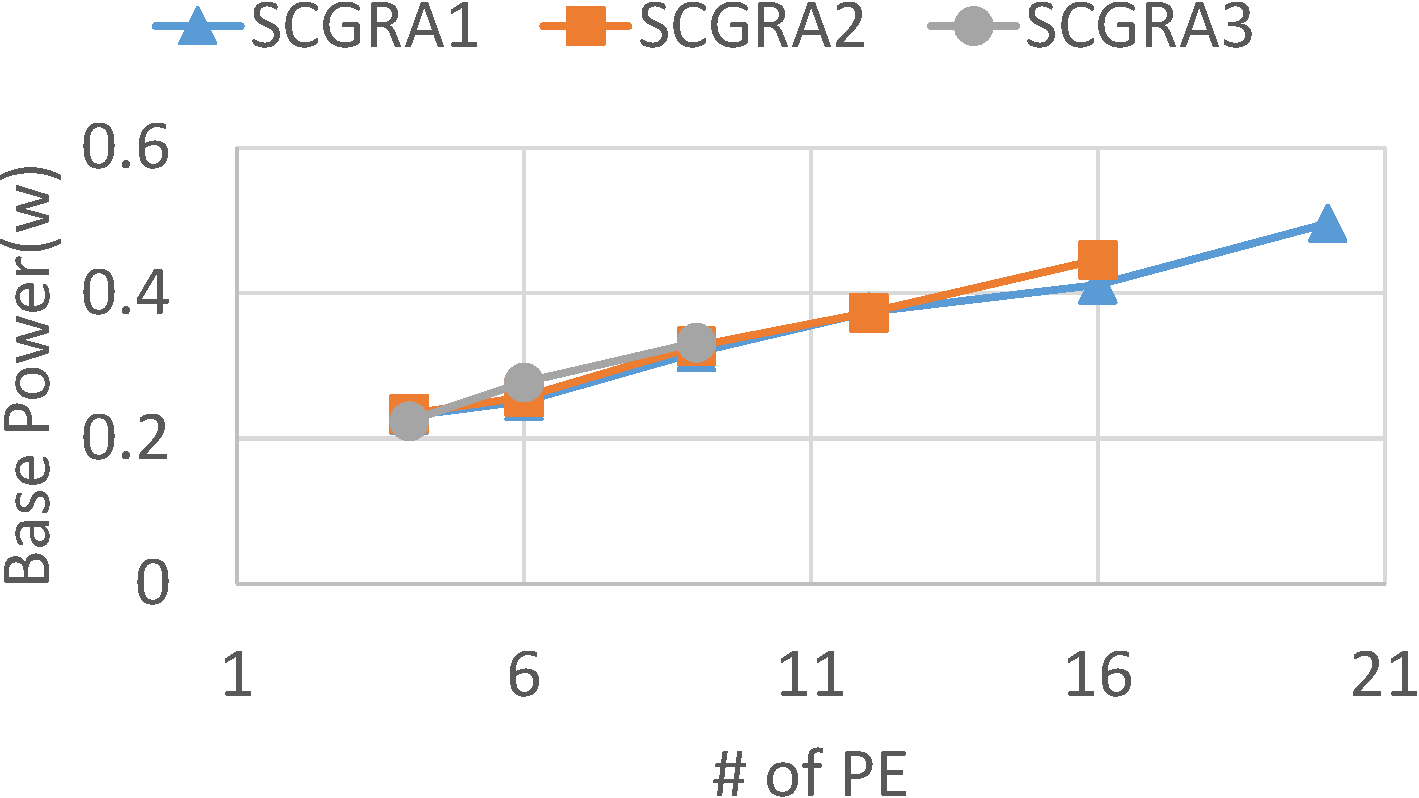
\includegraphics[width=0.4\textwidth]{Base-Power}
    }
    \subfigure[\label{fig:BRAM-Power}]{%
      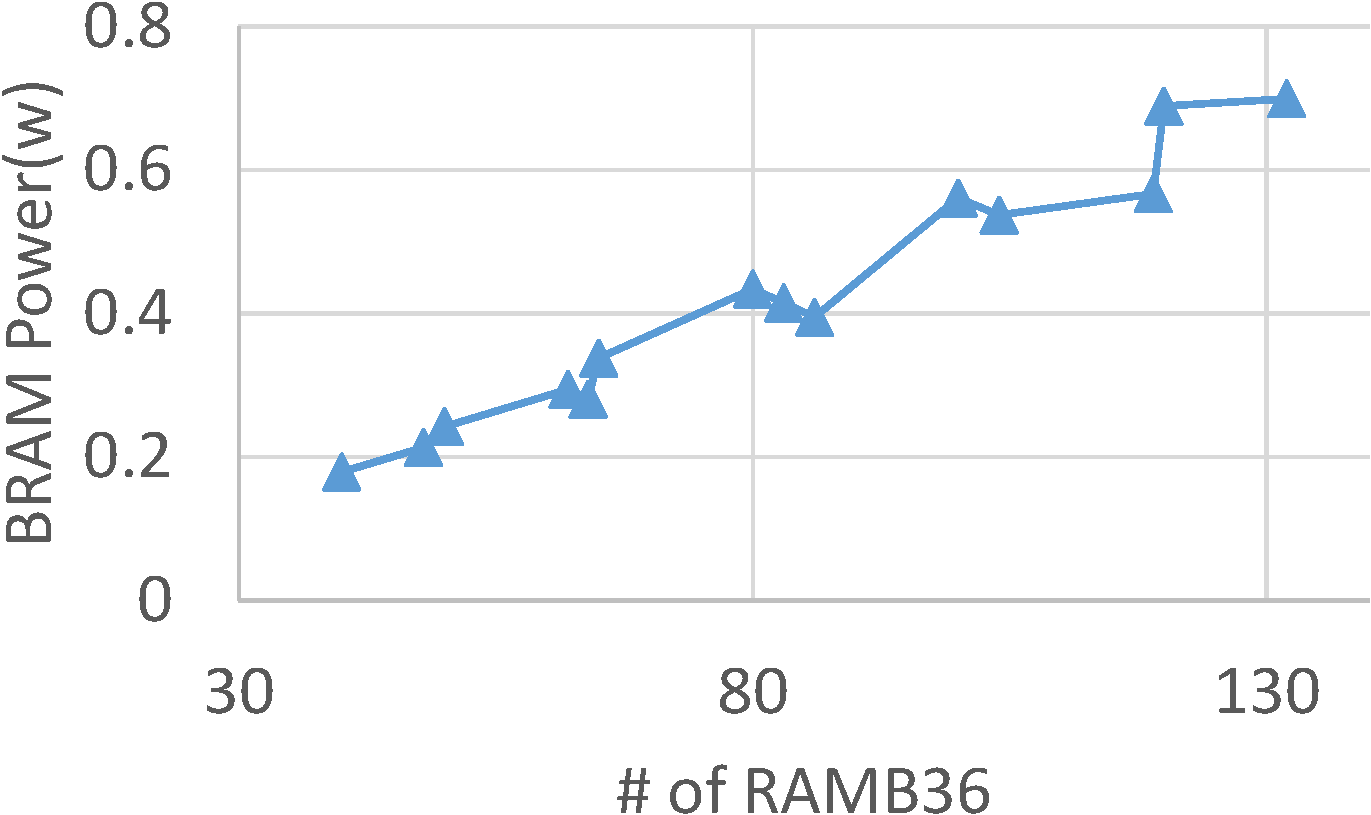
\includegraphics[width=0.4\textwidth]{BRAM-Power}
    }
    \caption{Power Consumption of the SCGRA Overlay Based FPGA Accelerators, (a) Base System Power Including DSP Power, Clock power, Signal Power, etc., (b) BRAM Power}
    \label{fig:SCGRA-Power}
\end{figure}

On top of the FPGA resource consumption and power consumption, the implementation frequency of the accelerators is also relatively predictable as shown in experiments in \chapref{chapter:overlay}. With all the highly predictable implementation features, it is convenient to further estimate the energy consumption and energy efficiency and present insight on the FPGA loop accelerator in early design stage. Although the experiments are still limited to Zedboard, it is believed that similar highly predictable implementation results can be observed on a different platform as the predictability comes from the regularity of the underlying SCGRA overlay. This is one of the advantages adopting SCGRA overlay for FPGA loop accelerator design compared to the design flow using conventional HDL or HLS which rarely guarantees the implementation details due to the extremely complex placing and routing process of the FPGA implementation.  

The data transfer between the accelerator and main memory is also very important to the FPGA loop accelerator customization. In this work, the communication latency is modeled based on DMA latency obtained from Zedboard. The FPGA accelerator implemented on programmable logic and the main memory may either communicate through a general purpose (GP) AXI port or a high performance AXI port, and the communication latency per word i.e. 32 bit data is presented in \figref{fig:dma-latency}. Despite the two different DMA engines, the basic trend of the communication cost per word is very similar. When the data transfer size is small, DMA communication cost per word is much larger due to the initial DMA transfer cost. When the data transfer size goes up, the initial DMA cost is amortized and communication cost per word is almost a constant. To estimate the data communication cost, a piece-wise linear function is used to model the DMA transfer. 

\begin{figure}[htb]
    \centering
    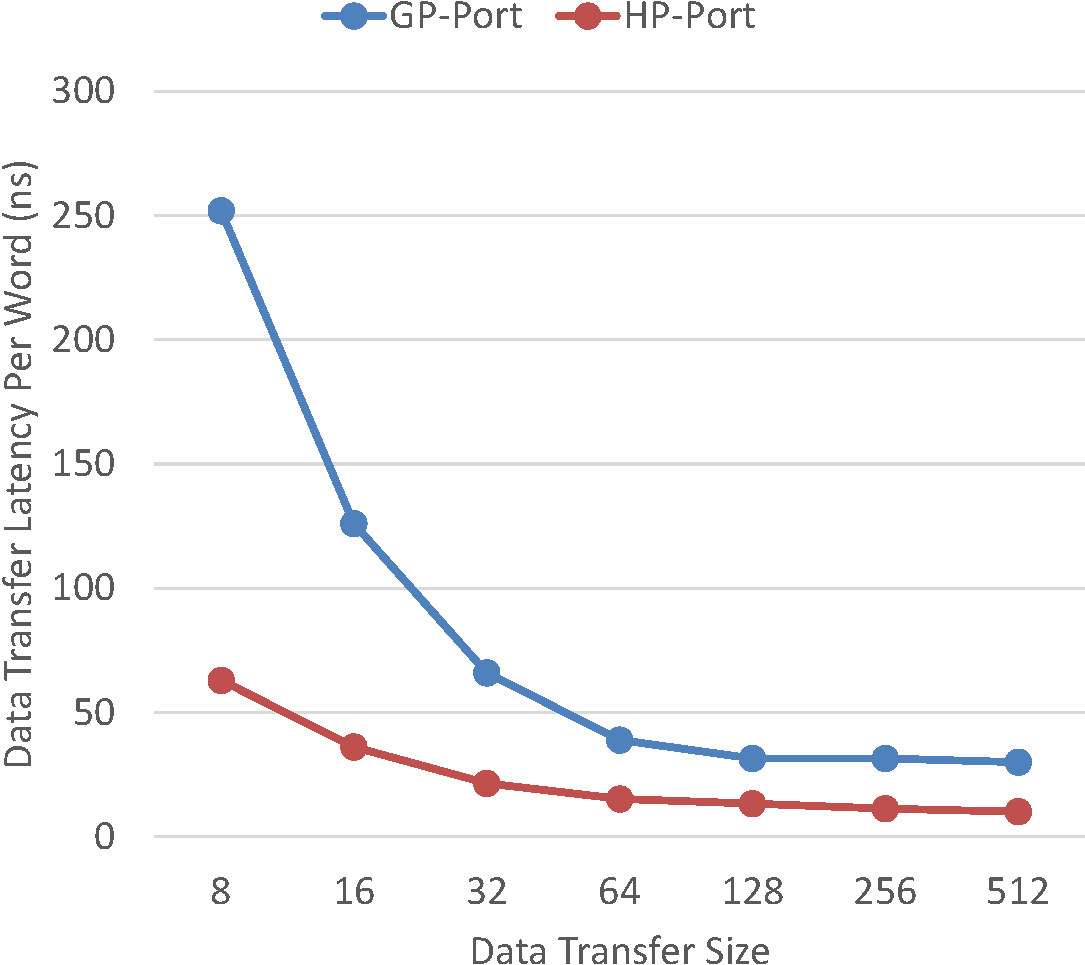
\includegraphics[width=0.6\textwidth]{dma-latency}
    \caption{Zedboard DMA Transfer Latency Per Word}
    \label{fig:dma-latency}
\end{figure}

According to the experiment, it can be found that the data transfer between FPGA accelerator and the main memory should be large enough to amortize the initial DMA cost, otherwise the communication cost can be 6X to 8X times larger which dramatically decreases the overall performance speedup achieved by the FPGA accelerator. This is also one of the major reasons that additional loop grouping strategy is adopted in QuickDough. 

